\begin{frame}{Synchronization of LoRa Transceivers}
  \begin{center}
    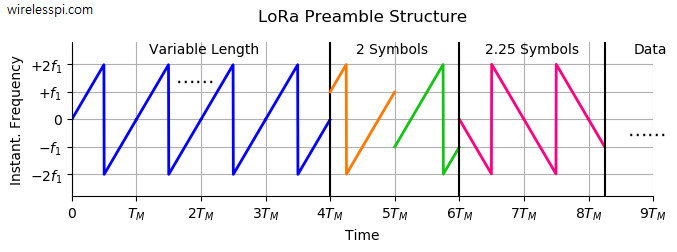
\includegraphics[width=0.65\textwidth]{material/figure-lora-preamble-structure}
  \end{center}
  \begin{itemize}
    \item Synchronization starts with an \alert{arbitrary amount $\ge 8$ of unmodulated up-chirps}, followed by
    \item \alert{two chirps} with a \alert{predefined modulation\footnote{\alert{LoRaWAN} uses \alert{up-chirp} as predefined modulation.}} encoding a network number, terminated by
    \item \alert{unmodulated down-chirps} that continuous for \alert{$2,25$ symbol times}.
  \end{itemize}
    \begin{description}[$\Rightarrow$]
      \item[$\Rightarrow$] The preamble \alert{total length} is \alert{$12,25$ symbols}.
      \item[$\Rightarrow$] Immediately after the synchronization sequence the \alert{data follows}.
    \end{description}
\end{frame}
